\UseRawInputEncoding
\documentclass[letterpaper]{aastex701}
\usepackage{graphicx}
\usepackage{hyperref}
\usepackage[margin=1in]{geometry}
\usepackage{float}
\usepackage{natbib}


\begin{document}

\title{Little Red Dot Density and Temperature Prediction Using Triplet Helium Strengths}

\author{Akshaj Vyas} \affiliation{Lake Travis High School} 
\email{what@what.com}

\author{Ian Bishop} 
\affiliation{idk} 
\email{what@what.com}

\date{July 2026}

\section{Introduction}

\subsection{Background}

%for later: change how we state a line to use lambda, for example, He I 10830A becomes He I lambda10830
% Cite OCEANS paper
Compared to previous astronomical telescopes, the James Webb Space Telescope (JWST) demonstrated a higher resolution and greater observational depth at infrared wavelengths than any previous space-based telescope. This led to the discovery of Little Red Dots (LRDs) within JWST deep-field images from the CEERS survey \citep{Finkelstein_2025}. LRDs are present in all JWST deep field images, especially at redshifts of  $4 < z < 9$. LRDs were deemed noteworthy due to a unique "v-shaped" spectral distribution, with opposite rest-UV and rest-optical slopes \citep{Matthee_2024} \citep{Kocevski_2025}. Further spectroscopy revealed the presence of unusual Balmer line broadening within the spectral distribution \citep{Kocevski_2025} \citep{Taylor_2025}. 

LRDs were originally hypothesized to be overmassive early-universe galaxies, though a contradiction arose with this idea, where the predicted stellar masses within the galaxies were unexpectedly high compared to prior observations \citep{Labbe2023}. Further disproving this early hypothesis, spectroscopic investigations demonstrated that the emissions of LRDs were dominated by supermassive black hole (SMBH) light \citep{Kocevski_2025} \citep{Taylor_2025}. The most recent studies have explained the broadening by introducing a dense cocoon of excited gas surrounding the LRD \citep{2025arXiv250316596N} \cite{Rusakov2026}.

Previous work has focused on Hydrogen I emission lines to estimate LRD physical properties. However, the properties of Helium lines show similar broadening and absorption features as Balmer lines, indicating that the excited gas has a significant effect on the emission of Helium lines \citet{Juod_balis_2024} \citet{Wang__2025} \citet{kokorev2025deepestglimpsedensegas}  \citet{de_Graaff_2025}. This work investigates the possibility of utilizing Helium lines to predict the temperature and density of the cocooning gas enshrouding LRDs.

\subsection{Goals}

To estimate the temperature and density of LRDs, we perform spectral analysis of four critical emission lines: He I $10830\AA$, H I $Pa\gamma$, He I $5876\AA$, and He I $7065\AA$. Additionally, we lay the foundation for future simulations which can provide significantly more accurate estimates of physical characteristics, through more precise models. Understanding the temperature and density of LRDs is critical to determining the structure of these objects, and could eventually result in a conclusive theory for LRDs.

\subsection{Helium}
%find sources explaining all of these concepts
The metastable He I helium line $10830\AA$ emerges when helium transitions from $1s2p^3P^\circ_J$ to $1s2s^3S_1$. The He I $10830\AA$ metastable transition is unique as its lower metastable level, known as the He I $2^3 S_1$ state, is substantially more stable than other non-ground state helium. This is due to the decay being forbidden by quantum mechanics, leading to an extremely low probability of transition. When isolated, a helium atom can remain in the $2^3 S_1$ state for about $7.8 \cdot 10^3s$ \citep{Sun2020-um}. This property of metastable helium creates a cycle between emission and absorption of free electrons, causing a strong correlation between the strength of the emission line and electron density. We take advantage of this property to accurately estimate the density of LRDs. 

We compare the He I $10830\AA$ line to the H I $Pa\gamma$ line due to its consistency among the LRD sample, and close proximity to $10830\AA$, which eliminates the requirement for dust correction.

% be sure to cite https://articles.adsabs.harvard.edu/pdf/1994ApJ...435..647I here (reminder for me)

As for the He I $5876\AA$ and $7065\AA$, these emerge when Helium transitions to $2^3S$ from the states $3^3D$ and $3^3S$, respectively. He I $7065\AA$ was chosen as it is highly sensitive to electron density. This is because represents a transition along the pathway to metastable Helium, indicating the transitions, and therefore the sensitivity to electron density, are correlated. He I $5876$ was chosen as it was the most common line among the sampled LRDs.


\begin{figure}[H]
    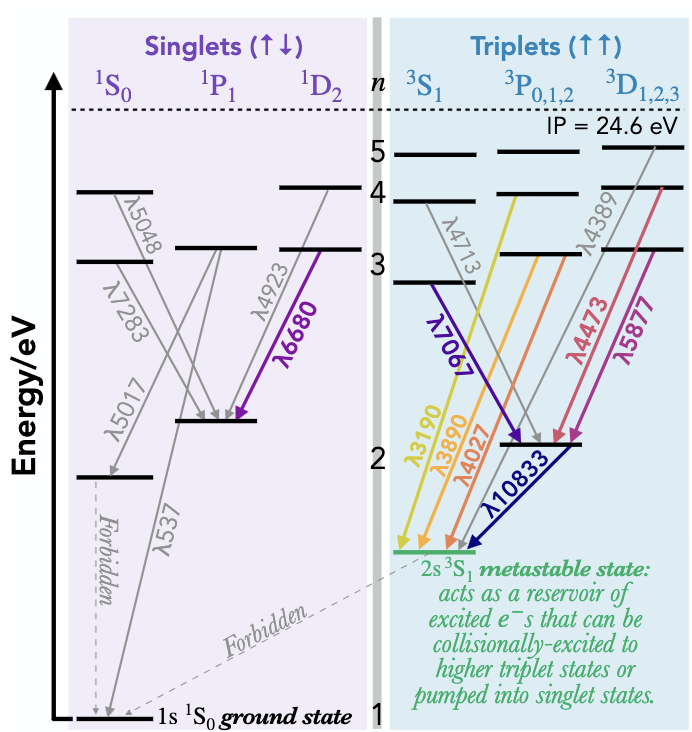
\includegraphics[width=10cm]{Helium_States.png}
    \centering
    \caption{Figure 3 from \citet{Berg_2026} describes the transition between every Helium state, and particularly emphasizes the longevity of the metastable state.}
\end{figure}

\section{Methods}

\subsection{Data}
%for Ian, talk about how the data used is medium resolution
The 1-dimensional extractions used for this work are courtesy of the OCEANS collaboration. The extractions utilized the NIRSpec instrument from the JWST, probing the rest-optical observed-IR light from the LRD. We configured the telescope to the high-resolution G235H and G395H gratings, both of which covered ranges in the single-digit microns.

For our metastable helium analysis, we pulled pre-calculated narrow and broad fluxes for the He I $\lambda10830$ line from \citet{Juod_balis_2024}, \citet{Wang__2025}, \citet{kokorev2025deepestglimpsedensegas}, and \citet{de_Graaff_2025}. We do this due to complexities involved with measuring this line, which are discussed more in the "Flux Measurement" section of this paper. This is also due to the rarity of these lines in LRDs, with only a handful exhibiting significant signs of the He I $\lambda10830$ line.

Before we performed spectral analysis, we cleaned the data to prepare it for Flux Measurement. First, we converted the units of $\mu$m to $\AA$ and $Jy$ (or $\mu Jy$) to $erg \cdot cm^{-2} s^{-1} \AA^{-1}$. This conversion leads to LiME providing integrated flux measurements in $erg \cdot cm^{-2} s^{-1}$. Next, we adjusted the wavelength for redshift using the formula $\lambda_{rest} = \frac{\lambda_{obs}}{1+z}$, where $z$ represents the redshift. The wavelength was corrected utilizing the Python library \texttt{NumPy} \citep{harris2020array}. Although the single-digit micron range exceeds the wavelength range of visible and near-infrared light, correcting for redshift reveals the appropriate emission lines primarily in the G395H grating.


\subsection{Flux Measurement}
%papers used for the He I 10830 line measurements:
%https://arxiv.org/pdf/2407.08643 
%https://arxiv.org/abs/2403.02304 
%https://arxiv.org/abs/2511.07515 
%https://arxiv.org/abs/2503.16600
% elaborate more on why 10830 is so complex
We use the Python library LiME (Line Measuring library) to measure fluxes \citet{LiMe_paper}. We measured narrow fluxes from the observed data for He I $5876\AA$, He I $7065\AA$, and H I $10941\AA$. Because He I $10830\AA$ had a complex line shape with broad and narrow emission superimposed with absorption, we used pre-aggregated tables from prior research papers \citep{Juod_balis_2024, Wang__2025, kokorev2025deepestglimpsedensegas, de_Graaff_2025} to avoid repeating the complicated work.

Next, we fit a continuum to the spectrum using a cubic equation. To eliminate emission lines from the continuum, we iteratively refit the cubic while clipping emission lines past a $\sigma$ threshold above the continuum. As the iterations progress, we gradually reduce the threshold from $3\sigma$ to $1\sigma$. Then, we performed line detection, where we utilized a neighbor comparison algorithm to detect all extrema relative to the continuum, and compared the detected extrema to LiME's internal database of known spectral lines. If a spectra excluded any of the lines, it was removed as a non-detection. The continuum fitting and line detection were implemented by LiME. However, tuning the parameters to the values mentioned was essential in order to achieve accurate line predictions. The accuracy of the line predictions was determined by visually inspecting the plots and ensuring most peaks and valleys were mapped to an appropriate emission line.

%we can change the name to something else later, helium analysis is just a temp name, same for metastable helium analysis
Next, we measured fluxes through profile fitting. For the He I $5876\AA$, $7065\AA$, and H I Pa$\gamma$ lines, the flux was best modeled by a Gaussian profile without broadening or blending. The Gaussian was fit through a least squares regression. We measured the flux by integrating over this Gaussian, taking into account the continuum as the floor for integration. The criteria for a false positive was a $3\sigma$ detection for Pa$\gamma\AA$ and a $2\sigma$ detection for other lines. Distributions which failed to meet this threshold were removed as non-detections.

% cite https://arxiv.org/abs/2403.02304 (please make better inline citation when final rpoduct)
For He I $10830\AA$, the fluxes were loaded from previous spectroscopic papers. While Wang et al precalculated the total flux, every other source provided only the narrow, broad and absorption flux. To find the total flux, the narrow and broad flux were added together, while the absorption was reintroduced into the line profile. We calculated the error based on formulas detailed in the next section. 

Finally, we calculated $\frac{F_{5876\AA}}{{F_{7065\AA}}}$, as well as $\frac{F_{10830\AA}}{{F_{10941\AA}}}$, and recorded these values for future comparison. The values were recorded and stored in a \texttt{.csv} file using the Python library \texttt{pandas} \citep{reback2020pandas}.

\begin{table}[H]
\begin{center}
\caption{Flux value table of each LRD with both the He I $5876\AA$ and $7065\AA$ line. Flux was measured in units of $10^{19} \cdot erg\cdot cm^{-2} \cdot s^{-1}$}
\begin{tabular}{|c|c|c|}
    \hline
    \centering
    \textbf{LRD} & He I $7065\AA$ flux & $5876\AA$ flux \\ \hline
    OCEANS 20504 P4 & 3.67 $\pm$ 0.72 & 8.49 $\pm$ 0.10 \\ \hline
    OCEANS 20504 P1 & 8.51 $\pm$ 1.14 & 4.79 $\pm$ 0.95 \\  \hline
    OCEANS 169045 P4 & 7.52 $\pm$ 0.68 & 3.84 $\pm$ 0.57 \\   \hline
    OCEANS 102364 P5 & 2.98 $\pm$ 0.83 & 2.96 $\pm$ 0.53 \\   \hline
\end{tabular}
\end{center}
\end{table}

\begin{table}[H]
\begin{center}
\caption{Flux value table of each LRD with both the He I $10830\AA$ and $Pa\gamma$ lines. Flux was measured in units of $10^{18} \cdot erg\cdot cm^{-2} \cdot s^{-1}$}
\begin{tabular}{|c|c|c|}
    \hline
    \centering
    \textbf{LRD} & He I $10830\AA$ flux & $Pa\gamma$ flux \\ \hline
    JADES 28074 G235M & $82.11^{+1.303}_{-1.400}$ & 22.1 $\pm$ 1.27 \\ \hline
    JADES 28074 G395M & $82.11^{+1.303}_{-1.400}$ & 21.2 $\pm$ 1.69 \\  \hline
    RUBIES 40579 G395M & $70^{+4}_{-3}$ & 40.5 $\pm$ 4.23 \\   \hline
    RUBIES 154183 G395M & $2.7^{+5.8}_{-5.8}$ & 2.74 $\pm$ 1.44 \\   \hline
    GLIMPSE 17775 G395M & $24.58^{+2.334}_{-2.334}$ & 5.16 $\pm$ 0.29 \\   \hline
\end{tabular}
\end{center}
\end{table}

\subsection{Flux Error Calculation}
%add any info about error calculation here, like the quadrature approach
The error propagation is derived from the LiME measurement, and represents the error of the fit. Flux error was calculated simultaneously with flux values. Whenever operations were performed on flux values, we performed the corresponding quadrature operation on error. For addition and subtraction, we use the following formula:

\[\sigma_z = \sqrt{\sigma_x^2+\sigma_y^2}\]

This formula was specifically used when adding the broad and narrow flux to calculate the total positive and negative error for He I $10830\AA$:

\[\sigma_{\mathrm{He,\,total}} = \sqrt{\sigma_{\mathrm{He,\,narrow}}^2 + \sigma_{\mathrm{He,\,broad}}^2}\]

For error derived from the multiplication or division of flux, we instead add the relative errors in quadrature:

\[\frac{\sigma_z}{z} = \sqrt{(\left(\frac{\sigma_x}{x}\right)^2+(\left(\frac{\sigma_y}{y}\right)^2}\]

We utilized this formula when calculating flux ratios between different flux measurements to calculate the total error of our ratios:

\[
\sigma_R = 
R\sqrt{\left(\frac{\sigma_{F_1}}{F_1}\right)^2 + 
\left(\frac{\sigma_{F_2}}{F_2}\right)^2}
\]

\subsection{Dust Correction}

We shifted the line fluxes to reverse the effects of dust extinction on the emission spectra. This applies only to the $5876\AA$ and $7065\AA$ emission lines. For the other ratio, the relative effect of dust extinction is minimal, since the wavelengths of He I $10830\AA$ and H I $Pa\gamma$ are adjacent. 

% https://iopscience.iop.org/article/10.3847/2041-8213/ae1955/pdf
We utilized the \texttt{astropy.dust\_extinction} library in Python to accomplish correction \citep{Gordon2024}. We chose a model called G24\_SMCAvg, representing conditions in the SMC (Small Magellanic Cloud) \citep{2024ApJ...970...51G}. This model was chosen as it was best representative of the low-metalicity conditions in the early universe. This provided a rough estimate for conditions in LRDs. The G24\_SMCAvg model requires $A_V$, the total visual extinction, to be passed in for a correct model. We calculated this value using Balmer decrements (defined as H$\alpha$ / H$\beta$) and a formula derived from \citet{2016ApJ...817L...9N}.

The color excess was calculated using this formula:
\[E(H\beta - H\alpha) = 2.5 \cdot log(\frac{(H\alpha/H\beta)_{obs}}{(H\alpha/H\beta)_{int}})\]

Then, we multiplied the color excess by the reddening curve to find the total visual extinction:
\[A_V = \frac{E(H\beta - H\alpha)}{k(\lambda_{H\beta}) - k(\lambda_{H\alpha})}\]

We passed $A_V$ into the model to obtain a correction factor for each flux value, which we divide the flux by to obtain the corrected values.

\subsection{Theoretical Predictions}

We used the Python library \texttt{pyneb} in order to generate theoretical predictions of emissivity ratios from density and temperature \citep{2015A&A...573A..42L}. To model a wide variety of LRD conditions, we chose a range of density logarithmically from $10^{5}$ to $10^{13}$ $cm^{-3}$, and a range of temperature linearly from 5000 $K$ and 25000 $K$. The ranges were both generated at resolutions of 100 steps, and were capped at these particular values since \texttt{pyneb} would lose precision and throw errors for values beyond this range. We computed the flux of He I $7065\AA$ and $5876\AA$ for each combination of temperature and density. Then, we calculated the ratio of these two values and stored them in a matrix.

Finally, we calculated the difference in flux between each place in the matrix and each observed flux value, recording the minimum difference for each observed flux. This allows us to find the temperature and density prediction closest to the observed flux.

\begin{table}[h]
\begin{center}
\caption{This is a temperature/density prediction table of each LRD, utilizing the $5876\AA$ and $7065\AA$ ratio.}
\begin{tabular}{|c|c|c|}
    \hline
    \centering
    \textbf{LRD} & Temperature ($K$) & Density $cm^{-3}$ \\ \hline
    OCEANS 20504 P4 & 9108 & $1 \cdot 10^{13}$ \\ \hline
    OCEANS 20504 P1 & 11840 & $2.29 \cdot 10^{7}$ \\  \hline
    OCEANS 169045 P4 & 9108 & $1 \cdot 10^{13}$ \\   \hline
    OCEANS 102364 P5 & 9108 & $1 \cdot 10^{13}$ \\   \hline
\end{tabular}
\end{center}
\end{table}

\subsection{Abundance Calculation}
%paper where the formula for flux ratio is from: https://arxiv.org/pdf/1309.0047
Using just the predictions given by \texttt{pyneb}, we are comparing two emission lines at a one-to-one ratio without taking into account the number of ions for each atom. This issue does not apply to the ratio between the He I $5876\AA$ and $7065\AA$ line though, as they both derive from triplet He I and thus have the same abundance. For this reason, we will focus on the ratio between the He I $10830\AA$ and H I Pa$\gamma$ lines.

In order to find the ratio between the flux of two emission lines, we must take into consideration two main components: the number of emitting ions and the emission efficiency of each ion. This can be seen in the following equation, which has been adapted for the He I $10830\AA$ and H I $10941\AA$ lines:

\[
\frac{F(\mathrm{He\,I\,\lambda10830})}{F(\mathrm{Pa\,\gamma})}
\approx
\frac{n(\mathrm{He^+})}{n\mathrm{(H^+)}}
\frac{\epsilon(\mathrm{He\,I\,\lambda10830})}{\epsilon(\mathrm{Pa\,\gamma})}
\]

Although there are other observational factors that affect the measured fluxes of these lines, they are removed from the equation because these factors affect the He I $\lambda10830$ and H I $\lambda10941$ lines similarly.

\texttt{pyneb} only gives us the emission portion of the above equation:

\[
R_{\mathrm{PyNeb}} = \frac{\epsilon(\mathrm{He\,I\,\lambda10830})}{\epsilon(\mathrm{Pa\,\gamma})}
\]

We still must account for the abundance of $\mathrm{He^+}$ and $\mathrm{H^+}$ to properly predict the flux ratio. To do this, we must measure the flux of a different helium line and hydrogen line. We found that the He I $\lambda7065$ and H $\alpha$ lines were the most consistently simultaneously observed lines in systems with He I $10830\AA$ emission, measuring the narrow component of each for consistency. Rearranging the above flux ratio equation and substituting these lines, we get the following:

\[
\frac{n(\mathrm{He^+})}{n\mathrm{(H^+)}}
\approx
\frac{F(\mathrm{He\,I\,\lambda7065})}{F(\mathrm{H\,\alpha})}
\frac{\epsilon(\mathrm{H\,\alpha})}{\epsilon(\mathrm{He\,I\,\lambda7065})}
\]

Here we run into an issue though: in order to calculate the emissivity needed to find the abundance, we need a given temperature and density, but in order to get that temperature and density, we need to calculate the flux ratios that require the abundance ratio. This creates a circular loop where each component relies on the other. 

For simplicity, we assume the abundance ratio here is approximately 0.01. We multiply each element in the Pyneb prediction matrix by this value to get a more reasonable result.

\section{Results}

\subsection{Metastable Flux}

Analysis of the spectra for each of the 4 LRDs revealed that the $Pa\gamma$ line was prominent in all 4, and while the metastable He I $10941\AA$ line wasn't measured directly from the spectra, it was very strong in all 5 observations. It is important to note, however, that these lines were still relatively weak compared to other major features of the spectra. 

The GLIMPSE 17775 g395m, JADES 28074 g235m, and JADES 28074 g395m observations displayed a strong fit by a Gaussian for the $Pa\gamma$ line. The RUBIES 40579 g395m and RUBIES 154183 g395m observations had more ambiguous results, with RUBIES 40579 showing signs of a blending, and RUBIES 154183 showing a detection close to the continuum.

\begin{figure}[H]
    \begin{minipage}{0.45\textwidth}
        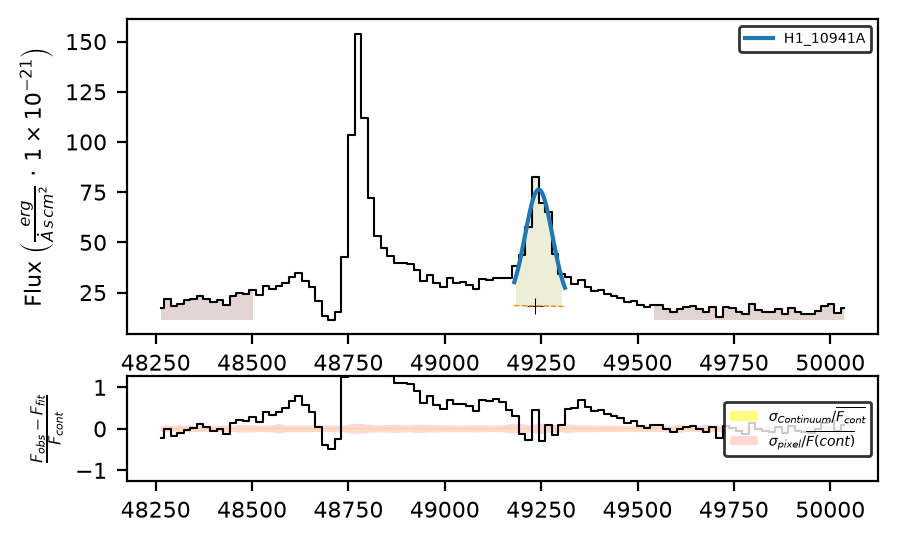
\includegraphics[trim={0 2.19cm 0 0},clip,width=9cm]{glimpse-obs02-v4_g395m-f290lp_9223_17775_fitted.png}
        \centering
        \caption{The fit of $Pa\gamma$ in GLIMPSE 17775 g395m. This is an example of a well-fit distribution. JADES 28074 g235m and JADES 28074 g395m yielded similar fits.}
    \end{minipage}\hfill
\end{figure}
\begin{figure}[H]
    \begin{minipage}{0.45\textwidth}
        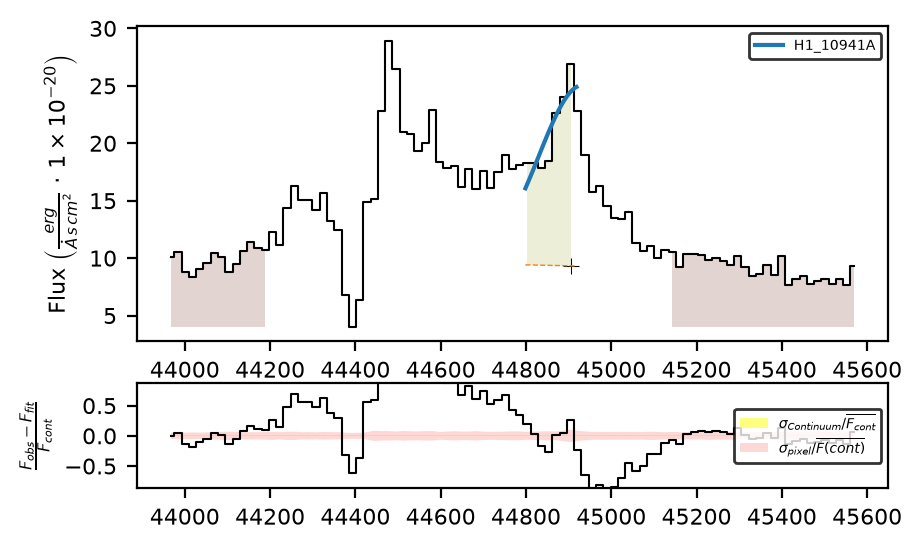
\includegraphics[trim={0 2.19cm 0 0},clip,width=9cm]{rubies-uds1-v4_g395m-f290lp_4233_40579_fitted.png}
        \centering
        \caption{The fit of $Pa\gamma$ in RUBIES 40579 g395m. This shows the result of a blended line, which is less favorable.}
    \end{minipage}\hfill
    \begin{minipage}{0.45\textwidth}
        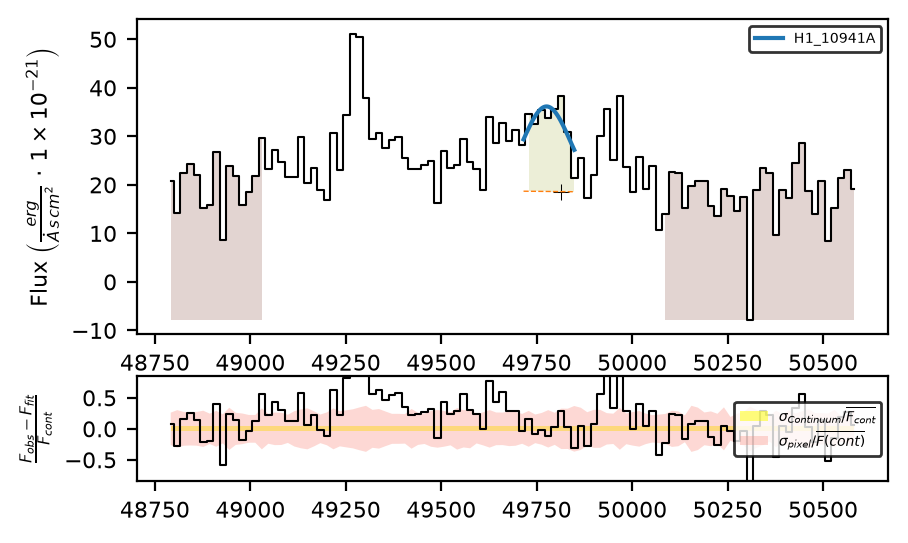
\includegraphics[trim={0 2.19cm 0 0},clip,width=9cm]{rubies-uds31-v4_g395m-f290lp_4233_154183_fitted.png}
        \centering
        \caption{The fit of $Pa\gamma$ in RUBIES 154183 g395m. Here we see the fit only barely above the continuum.}
    \end{minipage}\hfill
\end{figure}

Despite JADES 28074 g295m and JADES 28074 g395m being different observations, their flux measurements are relatively consistent.

Error between LRDs varied heavily, ranging between $\pm$2.5 in GLIMPSE 17775 to $^{+0.35}_{-0.34}$ in RUBIES 40579. Analysis of these LRDs' ratio $\frac{F_{He\,I\,10830\AA}}{{F_{Pa\gamma}}}$ reveal a mean of ~3.01, with a standard deviation of ~1.42. We also find that a median ratio of ~3.71 is exhibited. 

\subsubsection{Changes in Density Range}

Originally, we set the range for our Pyneb density predictions to be from $10^{5}$ to $10^{13}$. 

\begin{figure}[H]
    \begin{minipage}{0.45\textwidth}
        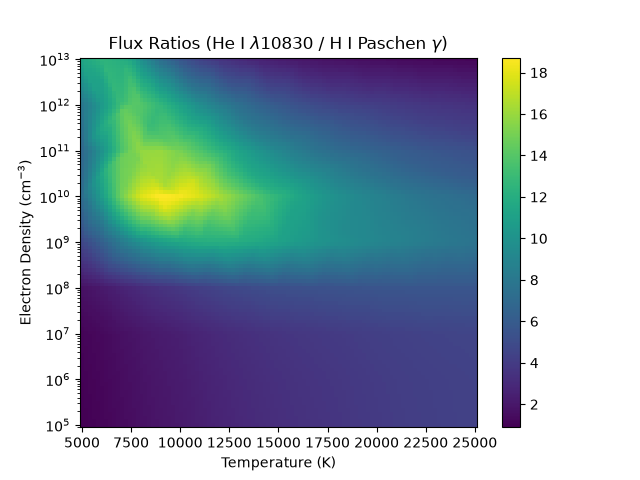
\includegraphics[trim={0 0 0 0},clip,width=9cm]{predicted-ratios-lower-range.png}
        \centering
        \caption{Flux ratio prediction matrix generated by Pyneb, with density scaled logarithmically. Both the lower density and the higher density regions show similarly low flux ratio values.}
    \end{minipage}\hfill
    \begin{minipage}{0.45\textwidth}
        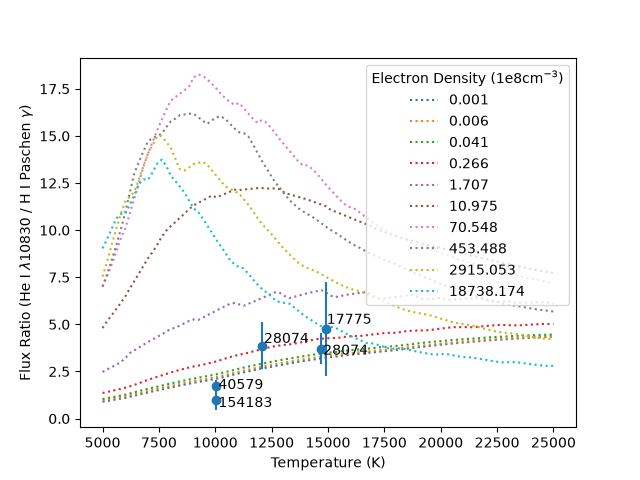
\includegraphics[trim={0 0 0 0},clip,width=9cm]{density-lines-lower-range.png}
        \centering
        \caption{Graph showing which density lines the flux ratios are best approximated by. Density lines are chosen based on a logarithmic scale similar to that of the Pyneb matrix. Notably, the measured flux ratios fall near the lower electron density lines.}
    \end{minipage}\hfill
\end{figure}

This, however, creates similarly low flux ratios for both the extreme high-density regions in the prediction matrix and the lower-density regions. This allows for the same low flux ratio LRDs to be misidentified as being low-density, which contradicts the results seen for our He I $7065\AA$ and He I $5876\AA$ lines (discussed in the next subsection). We can see this lower density misrepresentation in Figure 6, where the LRDs fall along the lower-density lines. To accommodate for this, we change the density range for which we create our prediction matrix, now using $10^{9}$ to $10^{15}$ to eliminate the lower regions with low flux ratio.

\begin{figure}[H]
    \begin{minipage}{0.45\textwidth}
        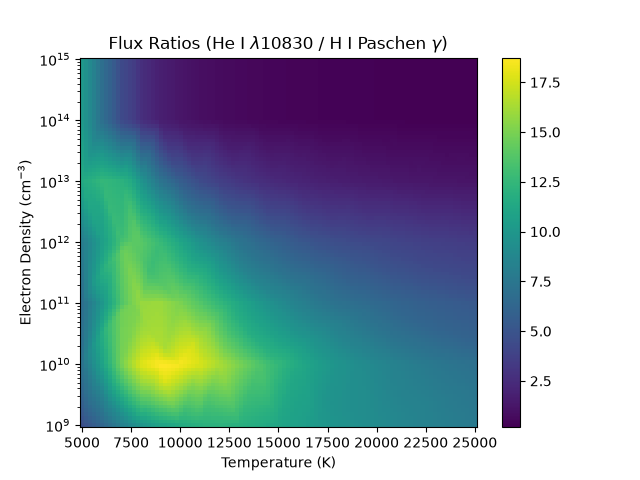
\includegraphics[trim={0 0 0 0},clip,width=9cm]{predicted-ratios-higher-range.png}
        \centering
        \caption{Flux ratio prediction matrix generated by Pyneb, with density scaled logarithmically. Here we see that now only the higher density region has areas of low flux ratio.}
    \end{minipage}\hfill
    \begin{minipage}{0.45\textwidth}
        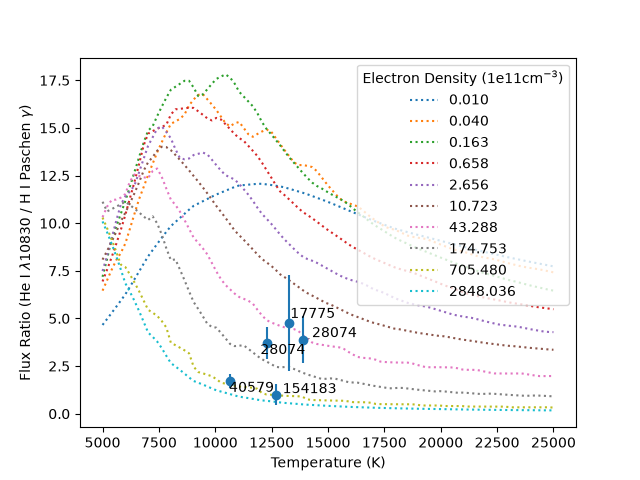
\includegraphics[trim={0 0 0 0},clip,width=9cm]{density-lines-higher-range.png}
        \centering
        \caption{Graph showing which density lines the flux ratios are best approximated by. Density lines are chosen based on a logarithmic scale similar to that of the Pyneb matrix. Here, the LRDs now reveal themselves to be closer to the extreme high-density lines.}
    \end{minipage}\hfill
\end{figure}

Using this adjusted density range, we now find that the results become more in line with those seen for the He I $7065\AA$ and $5876\AA$ lines (discussed in the next subsection), where the LRDs exhibit signs of extremely high density. 

\subsection{Other Flux}

The spectra of the LRDs revealed that He I $5876\AA$ and $7065\AA$ were relatively weak compared to the major features of the spectra, such as Balmer breaks. Additionally, only 30\% of the observed LRDs exhibited statistically significant observations of both fluxes. However, He I $5876\AA$ was detected more commonly than He I $7065\AA$.

Despite their small presence within the spectra, most emission lines were well-fit by a Gaussian. However, many lines were ambiguous detections, often located only marginally above the continuum. The presence of poor fits was reflected in the calculated flux values. For instance, the flux error peaked at 33\% for OCEANS 102364, with a sigma confidence of only $3.03\sigma$.

\begin{figure}[H]
    \begin{minipage}{0.45\textwidth}
        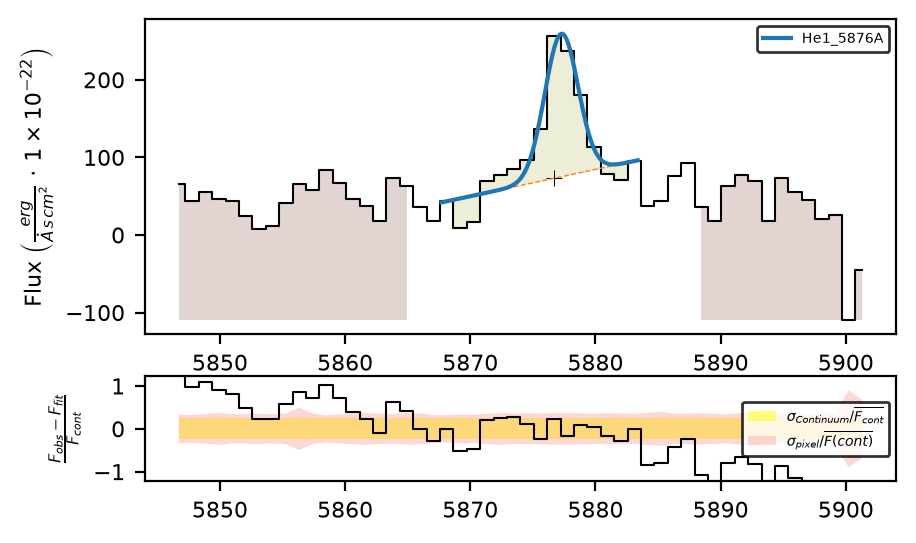
\includegraphics[trim={0 2.19cm 0 0},clip,width=9cm]{profile-395_000169045_P4-He1_5876A.png}
        \centering
        \caption{The fit of He I $5876\AA$ in OCEANS 169045. This is an example of a well-fit distribution.}
    \end{minipage}\hfill
    \begin{minipage}{0.45\textwidth}
       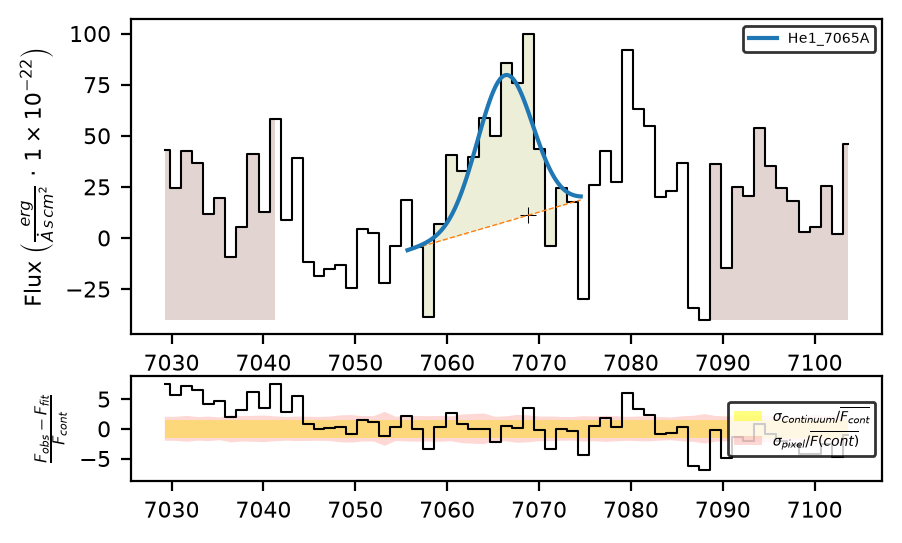
\includegraphics[trim={0 2.19cm 0 0},clip,width=9cm]{profile-395_000102364_P5-He1_7065A.png}
        \centering
        \caption{The fit of He I $7065\AA$ in OCEANS 102364. This is an example of a poor fit, as evidenced by the peak of the emission line being barely above the surrounding continuum.}
    \end{minipage}
\end{figure}

Another intriguing observation was the variability between different observations of OCEANS 20504. For instance, the P4 \footnote[1]{P4 (short for pointing 4) denotes the number of the observation.} observation, exhibited the least significant error and was situated considerably below the other data. However, the other observation of OCEANS 020504, the P1 observation, was closer to the other data points and had a prominent error.

The ratio $\frac{F_{5876\AA}}{{F_{7065\AA}}}$ exhibited a median of around  1.39, with a standard deviation of 0.62. The values ranged from as low as 0.43 to as high as 1.96. All flux ratios except OCEANS 20504's P4 observation far exceeded Pyneb's emissivity predictions. Pyneb's emissivity predictions exhibited a maximum of 1, even at densities of $10^{11} cm^{-3}$. Consequently, this indicates the presence of extremely dense areas  $> 10^{13} cm^{-3}$.

% I need to ask Kelcey where she got 10000 K from, cuz i gotta cite the fact that its a consensus
% i also have to verify the 10521 number as it seems outdated to me (using a previous version of pyneb_analysis.py)
Considering temperature predictions, the average predicted temperature was $10521 K$, close to the hypothesized value of $\sim 10000 \textrm{K}$ \citep{naidu2025blackholestarreveals}. However, temperature predictions and density predictions often varied significantly when modifying the range of temperature. In order to prevent such inconsistencies, we manually limited the range of predicted temperature to a window of $3000 K$ around $10000 K$, which provided more consistent density predictions and are reflective of the temperatures of LRDs implied by other observations. %(check whether kelcey approves of our method)

\subsubsection{Flux Corrections from Dust Extinction}

As a consequence of dust correction, all flux values significantly decreased, with the average moving from 1.29 to 0.78. However, one outlier continued to persist: OCEANS 169045 continued to emit 1.65 flux despite dust correction. Despite this anomaly, the predictions of \texttt{pyneb} were overall more accurate, causing the density predictions to be situated around $10^{11}-10^{12}$ for most LRDs. Additionally, the average temperature predictions reduced slightly to $9010 K$. The plots below were created by the Python library \texttt{matplotlib} \citep{Hunter:2007}.

\begin{figure}[H]
    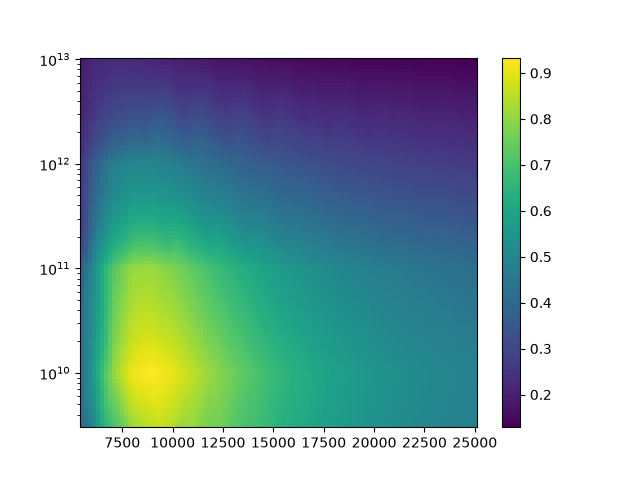
\includegraphics[width=10cm]{pyneb_matrix.png}
    \centering
    \caption{A plot of the matrix generated by Pyneb.}
\end{figure}

\begin{figure}[H]
    \begin{minipage}{0.45\textwidth}
        \centering
        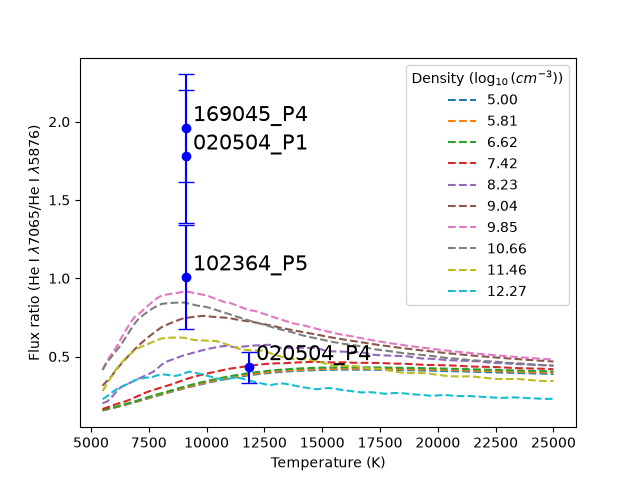
\includegraphics[width=0.9\textwidth]{final_plot.png} % first figure itself
        \caption{A plot of LRDs and their temperature and emissivity ratios compared to different lines of constant density.}
    \end{minipage}\hfill
    \begin{minipage}{0.45\textwidth}
       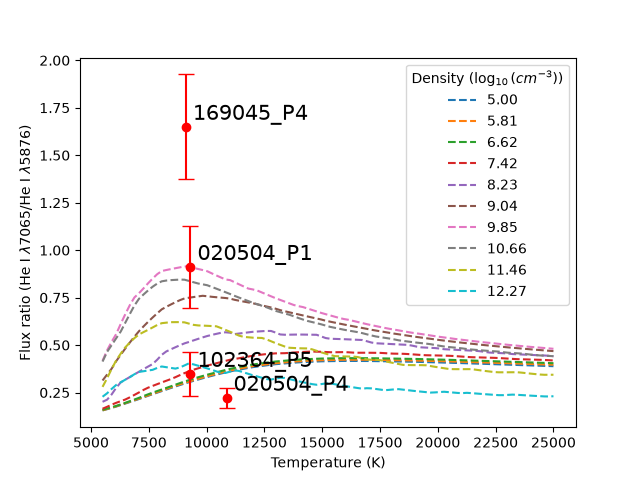
\includegraphics[width=0.9\textwidth]{final_plot_dust_correction.png}
        \centering
        \caption{A plot of LRDs and their temperature and emissivity ratios compared to different lines of constant density. This time, the emissivity ratios are adjusted for dust correction.}
    \end{minipage}
\end{figure}



\section{Discussion}

% https://arxiv.org/html/2512.03239v1 cite this


% cite https://ui.adsabs.harvard.edu/abs/2000MNRAS.315..791S/abstract

% https://arxiv.org/abs/2606.31515

\subsection{Importance of Dust Correction}

As mentioned in the Results section, the flux ratios between $7065\AA$ and $5876\AA$ were excessively high without dust correction, with the emission of $7065\AA$ displaying two times the flux as $5876\AA$ in one scenario. However, the abnormal flux values is attributable to the fact that dust extinction amplifies the longer wavelength, $7065\AA$, stronger than the shorter wavelength, $5876\AA$. Correcting this dust extinction reduces the flux ratios and significantly increases concordance with theoretical predictions. Interestingly, dust correction does not completely resolve the problem of inaccurate flux, as several outliers continue to persist past Pyneb's prediction bounds. 

\subsection{Limitations of Models}
% I accidentally removed a comment here oops, would you be able to add it back? I believe it was about inaccurate flux
% https://www.aanda.org/articles/aa/full_html/2015/01/aa23152-13/aa23152-13.html
To reiterate, LRDs are hypothesized to contain SMBHs which are surrounded by a highly dense region of gas. The density estimates reveal the gas exhibits a density of at least $10^{10} cm^{-3}$, strongly evidencing the presence of an external dense medium. This medium is likely to be optically thick and have strong collisional effects, due to the high density observed.

% find sources to support this, i had them but i lost them
% please also explain why optically thick matters
Two main drawbacks exist when using Pyneb to measure LRD Helium fluxes. First, Helium is treated as a recombination line within \texttt{pyneb}, where collisions are assumed to have minimal effect on emissivity. Second, the high density implies an optically thick region, while Pyneb assumes an optically thin medium. One option to resolve these assumptions, and therefore reconcile agreement with experimental data, is to augment radiative transfer code to analyze collisional effects. The library \texttt{CLOUDY} in Python could simulate more representative physics and will be the subject of future work.

\subsection{Low Detection Rate}

Another unique observation from this data is the low detection rate among the LRDs for this ratio. This is in part due to the rarity of the $7065\AA$ line, which acts as the bottleneck for detection. Increased observational depth could increase the significance of the detections and recover lines in more sources. Additionally, extending the wavelength range of observation could additionally reveal Helium lines in sources where there was no detection.

\section{Conclusions}

The goal of this study was to probe the density and temperature of LRDs using Helium emission spectra. The findings indicate a moderately effective probe, capable of restricting densities to a range of $\geq 10^{11}-10^{12} cm^{-3}$. However, specific density amounts varied widely among different LRDs, with some vastly exceeding predictions. The application of dust correction was critical to arriving at reasonable results, as values significantly exceeded the theoretical predictions when it was not applied. As for temperatures, most LRDs were well-fit near the consensus of $10000 K$, although the mean slightly decreased once dust correction was applied. The high densities indicate the presence of an enshrouded supermassive black hole within the LRD, largely reaffirming the existing theory. 

However, many improvements to these research methods exist, such as increased observational depth within the measurements to improve flux accuracy and expanded wavelength coverage to discover more metastable Helium lines. The comparison of the observed flux ratio to theoretical Pyneb predictions imply that more advanced modeling techniques are needed to reproduce the observed high ratios. One software tool which can accopmplish this is the Python library \texttt{CLOUDY}, which takes into account the optical depth of the measurement alongside collisional effects within the cocooning gas.

\section{Acknowledgements}

We would like to acknowledge Kelcey Davis due to her extensive feedback during the writing process, alongside her assistance in debugging our codebase. This work was completed at a research internship for the Institute for Computing in Research.

\bibliography{main}{}
\bibliographystyle{aasjournalv7}

\end{document}